\documentclass[a4paper,11pt]{article}

% --- Lenguaje y Fuentes ---
\usepackage[spanish, es-noshorthands]{babel}
\usepackage[T1]{fontenc}
\usepackage[sfdefault, scaled=.85]{FiraSans} 
\usepackage{newtxsf} % Matemáticas en sans-serif

% --- Geometría y Estilo de Página ---
\usepackage[left=3cm, right=3cm, top=2cm, bottom=3cm]{geometry}
\usepackage{fancyhdr}
\setlength{\headheight}{14.5pt} % Ajustado ligeramente para evitar warnings
\usepackage{titlesec}
\usepackage{multicol}

% --- Matemáticas y Gráficos ---
\usepackage{amsmath, amssymb, amsfonts}
\usepackage{cancel}
\usepackage{graphicx}
\usepackage{tikz}
\usepackage{float}
\usepackage{subcaption}
\usepackage{booktabs} % Para tablas profesionales

% --- Programación (Usando listings para evitar problemas con shell-escape) ---
\usepackage{listings}
\usepackage{xcolor}

% --- Referencias y Enlaces ---
\usepackage[hidelinks]{hyperref}
\usepackage{url}
% Cambia [authoryear] por [numbers]
\usepackage[numbers]{natbib} 
\bibliographystyle{plainnat}

% --- Configuración de Colores y Estilos ---
\definecolor{RoyalBlue}{rgb}{0.121, 0.239, 0.471}
\definecolor{backcolour}{rgb}{0.95, 0.95, 0.92}
\definecolor{codegreen}{rgb}{0,0.6,0}

\titleformat{\section}{\color{RoyalBlue}\normalfont\Large\bfseries}{\thesection.}{1em}{}
\titleformat{\subsection}{\color{RoyalBlue}\normalfont\large\bfseries}{\thesubsection.}{1em}{}

\lstset{
    language=Python,
    backgroundcolor=\color{backcolour},
    basicstyle=\ttfamily\small,
    keywordstyle=\color{blue},
    commentstyle=\color{codegreen},
    stringstyle=\color{red},
    breaklines=true,
    showstringspaces=false
}

% --- Encabezado y Pie de Página ---
\pagestyle{fancy}
\fancyhf{}
\fancyhead[L]{\footnotesize Universidad Nacional de Colombia}
\fancyhead[R]{\footnotesize Sede Bogotá}
\fancyfoot[L]{\footnotesize Modelación Matemática}
\fancyfoot[C]{\thepage}
\fancyfoot[R]{\footnotesize Actividad Teórica}
\renewcommand{\footrulewidth}{0.4pt}

\begin{document}

\begin{titlepage}
    \begin{center}
        % Asegúrate de que la carpeta y el archivo existan
        
\includegraphics[width=0.3\textwidth]{Portada/EscudoUN} 
\vspace{3.5cm}\vspace{3.5cm}

{\huge \textbf{Modelación Matemática - Gradientes (Sesion Teorica)}}\\[3cm]


{\Large \textbf{Nicolás Felipe Godoy Alarcón-1013113408}}\\[8cm]


\small
Universidad Nacional de Colombia\\
Facultad de Ingeniería\\
Bogotá D.C, Colombia\\
2025
    \end{center}
\end{titlepage}

\vspace{0.5cm}

% Los archivos Desarrollo.tex y Referencias.tex deben estar en la misma carpeta
\section*{Actividad}
Considerando la información presentada en la sesión del Miércoles 4 de Marzo (incluyendo la disponible en los videos recomendados en clase), para cada uno de los siguientes campos escalares $ f(x,y) $ produzca:
\begin{itemize}
    \item Un desarrollo hecho a mano del calculo del gradiente del campo escalar, $ \nabla  f(x,y) $ 
    \item El cálculo manual del gradiente en cuatro (4) puntos diferentes del plano $xy$
    \item Una representación visual del campo escalar de la función como gráfico de superficie usando \texttt{matplotlib}
    \item Una representación visual del campo vectorial $ \nabla  f(x,y) $ usando también \texttt{matplotlib}(por ejemplo usando \texttt{pyplot.quiver}
\end{itemize}
Las funciones son:
\begin{enumerate}
    \item $ f(x,y) = x^3-y^3 $
    \item $ f(x,y) = -x^3+y^3 $
    \item $ f(x,y) = x^2 y^2 -\sin{(xy)}$
    \item $ f(x,y) = \sin{(x)}\cos{(y)} -\cos{(y^2)}$
    \item $ f(x,y) = x^3+4x^2y - 5xy^2-y^3  $
    \item $ f(x,y) = \cos{(x^3)} + 4\sin{(x^2)}\cos{(y)}-5xy^2+y^3 $
\end{enumerate}
\section*{Solución}
\subsection*{Contexto y Teoría}
Lo más relevante que se puede añadir para el calculo de gradientes es entender la diferencia de una función escalar y una función vectorial, esto debido a que como se entiende una función escalar es una función que puede recibir 1, 2, 3, 4 o la cantidad de parámetros que se desee y el resultado sera un escalar, o sea un número, por ejemplo:
\[ f(x,y) = x^2 + y^2,\quad x,y \in \mathbb{R}\]
Si nos damos cuenta es una función que recibe dos números reales y nos devuelve un número real, se puede ver como una "Transformación"  definida como $T: \mathbb{R}^2 \rightarrow \mathbb{R}$, es como realizar un mapeo del plano  cartesiano hacía la recta de los números reales, en este caso el ejemplo que utilizamos se trata de un paraboloide (Dentro del código se presenta la forma de visualizar esta figura).
\subsubsection*{Operador $\nabla$}
El operador Nabla, representado por el símbolo $\nabla$, es un operador bastante interesante, ya que nos va a ayudar a definir operaciones como el rotacional y la divergencia. Pero antes de ello, vamos a utilizarlo para definir el gradiente. Más allá de lo teorico, una forma util de reconocerlo y usarlo es verlo de la forma \[ \nabla = \left(\dfrac{\partial}{\partial x}, \dfrac{\partial}{\partial y}\right) ; \quad \text{Cuando se haga referencia en el contexto de $\mathbb{R}^2$ (2 variables)}\]
\[
\nabla = \left(\frac{\partial}{\partial x}, \frac{\partial}{\partial y}, \frac{\partial}{\partial z}\right),
\quad \text{cuando se haga referencia en } \mathbb{R}^3 \;.
\]
Utilizando lo conocido en los cursos de Algebra Lineal podríamos darnos cuenta que cuando hacemos referencia a una operación como $ \nabla  f(x,y) $ estamos remitiendonos al producto escalar, esto resulta en un vector de $\mathbb{R}^n$ n siendo la DIMENSIÓN de $\nabla$, si nos damos cuenta lo que estamos haciendo es llevar una función escalar a una función vectorial (funcion de $\mathbb{R}^n\rightarrow\mathbb{R}^n$) note que lleva de n a n, esto debido a que el gradiente tiene la dimension que necesitemos dependiendo del contexto, si tenemos 5 variables, podemos hacer un gradiente con estas 5 variables.
\subsection*{Resolución Gradientes y Evaluación en 4 puntos del plano cartesiano (A mano)}
\begin{figure}[H]
\centering
\includegraphics[width=\linewidth,page=1]{Images/A_Mano.pdf}
\caption{Desarrollo manual del cálculo del gradiente y análisis de punto en el plano (parte 1).}
\end{figure}

\begin{figure}[H]
\centering
\includegraphics[width=\linewidth,page=2]{Images/A_Mano.pdf}
\caption{Desarrollo manual del cálculo del gradiente y análisis de punto en el plano (parte 2).}
\end{figure}
\subsection*{Código Python y Gráficas}

Las siguientes visualizaciones fueron generadas utilizando Python y la biblioteca \texttt{matplotlib}. 
Para cada función se presenta el gráfico de superficie correspondiente al campo escalar y una representación del campo vectorial del gradiente.
\begin{lstlisting}[language=Python]
import numpy as np
import matplotlib.pyplot as plt
from mpl_toolkits import mplot3d

\end{lstlisting}
\subsubsection*{Gráficos superficies}
\begin{enumerate}
    \item $ f(x,y) = x^3-y^3 $
    \item $f(x,y) = -x^3+y^3$
    \item $ f(x,y) = x^2 y^2 -\sin{(xy)}$
    \item $ f(x,y) = \sin{(x)}\cos{(y)} -\cos{(y^2)}$
    \item $ f(x,y) = x^3+4x^2y - 5xy^2-y^3  $
    \item $ f(x,y) = \cos{(x^3)} + 4\sin{(x^2)}\cos{(y)}-5xy^2+y^3 $
\end{enumerate}
Por comodidad se presentan a continuación los gráficos de los campos vectoriales resultantes.
\subsubsection*{Gráficos Gradientes}
\begin{enumerate}
    \item $ \nabla f(x,y) = \left(3x^2 , -3y^2 \right) $
    \item $ \nabla f(x,y) = \left(-3x^2 , 3y^2 \right) $
    \item $ \nabla f(x,y) = \left(2xy^2-y\cos(xy) , 2x^2y-x\cos(xy) \right) $
    \item $ \nabla f(x,y) = \left(\cos(x)\cos(y), 2ysin(y^2)-\sin(x)\sin(y) \right) $
    \item $ \nabla f(x,y) = \left(3x^2+8xy-5y^2, 4x^2 -10xy - 3y^2\right) $
    \item $ \nabla f(x,y) = \left(-3x^2sin(x^3) + 8xcos(x^2)\cos(y) - 5y^2, -4sin(x^2)\sin(y)-10xy + 3y^2\right) $
\end{enumerate}

\begin{lstlisting}[language=Python]
# 1. Definimos los ejes (vectores 1D)
range_val = np.linspace(-20, 20, 50)

# 2. CREAMOS LA MALLA
x = np.outer(np.linspace(-3, 3, 100), np.ones(100))
#Vector Transpuesta
y = x.copy().T
# 3. Calculamos Z usando las matrices
z = x**3 - y**3

# 4. Graficamos (usando una proyeccion 3D)
fig, ax = plt.figure(figsize=(10, 8)), plt.axes(projection='3d') # Importante definir que es 3D
ax.plot_surface(x, y, z, cmap='inferno')
ax.view_init(elev=10, azim=90)
ax.set_title(r"1. $f(x,y) = x^3 - y^3$", fontsize=16, color='navy', pad=20)
fig.savefig('Ejercicio_1_Escalar.png', dpi=150, bbox_inches='tight')
plt.show()
\end{lstlisting}
\begin{figure}[H]
    \centering
    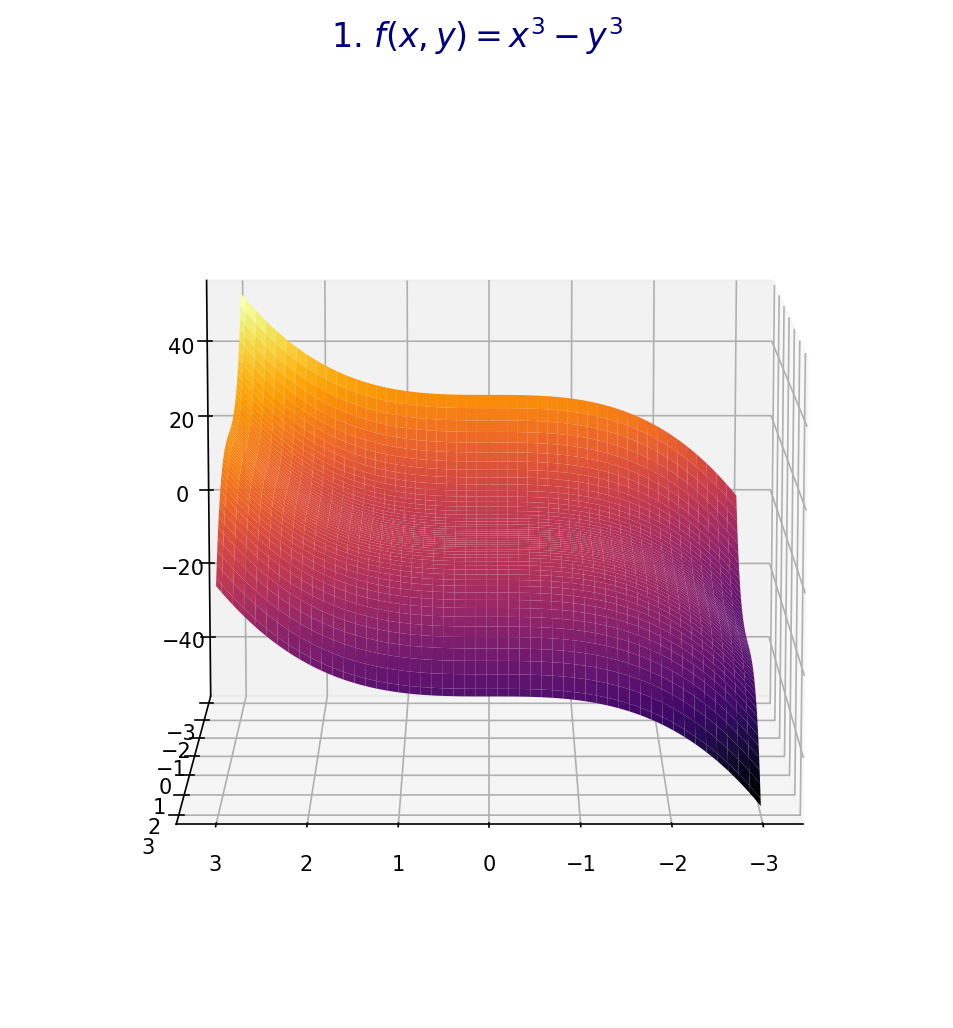
\includegraphics[width=0.65\linewidth]{Images/Ejercicio_1_Escalar.png}
    \caption{Función Escalar 1.}
    \label{fig:Esc1}
\end{figure}
\begin{lstlisting}[language=Python]
# 1D arrays
x = np.arange(-5,5,0.5)
y = np.arange(-5,5,0.5)

# Meshgrid
X,Y = np.meshgrid(x,y)

# Assign vector directions
fx = 3*X**2
fy = -3*Y**2

# Depict illustration
fig = plt.figure(figsize=(10, 10))
plt.streamplot(X,Y,fx,fy, density=1.4, linewidth=None, color='#44C3E3')
plt.title(r'1. $\nabla f(x,y) = \left(3x^2 , -3y^2 \right) $')

# Show plot with grid
plt.grid()
fig.savefig('Ejercicio_1_Vectorial.png', dpi=150, bbox_inches='tight')

plt.show()
\end{lstlisting}
\begin{figure}[H]
    \centering
    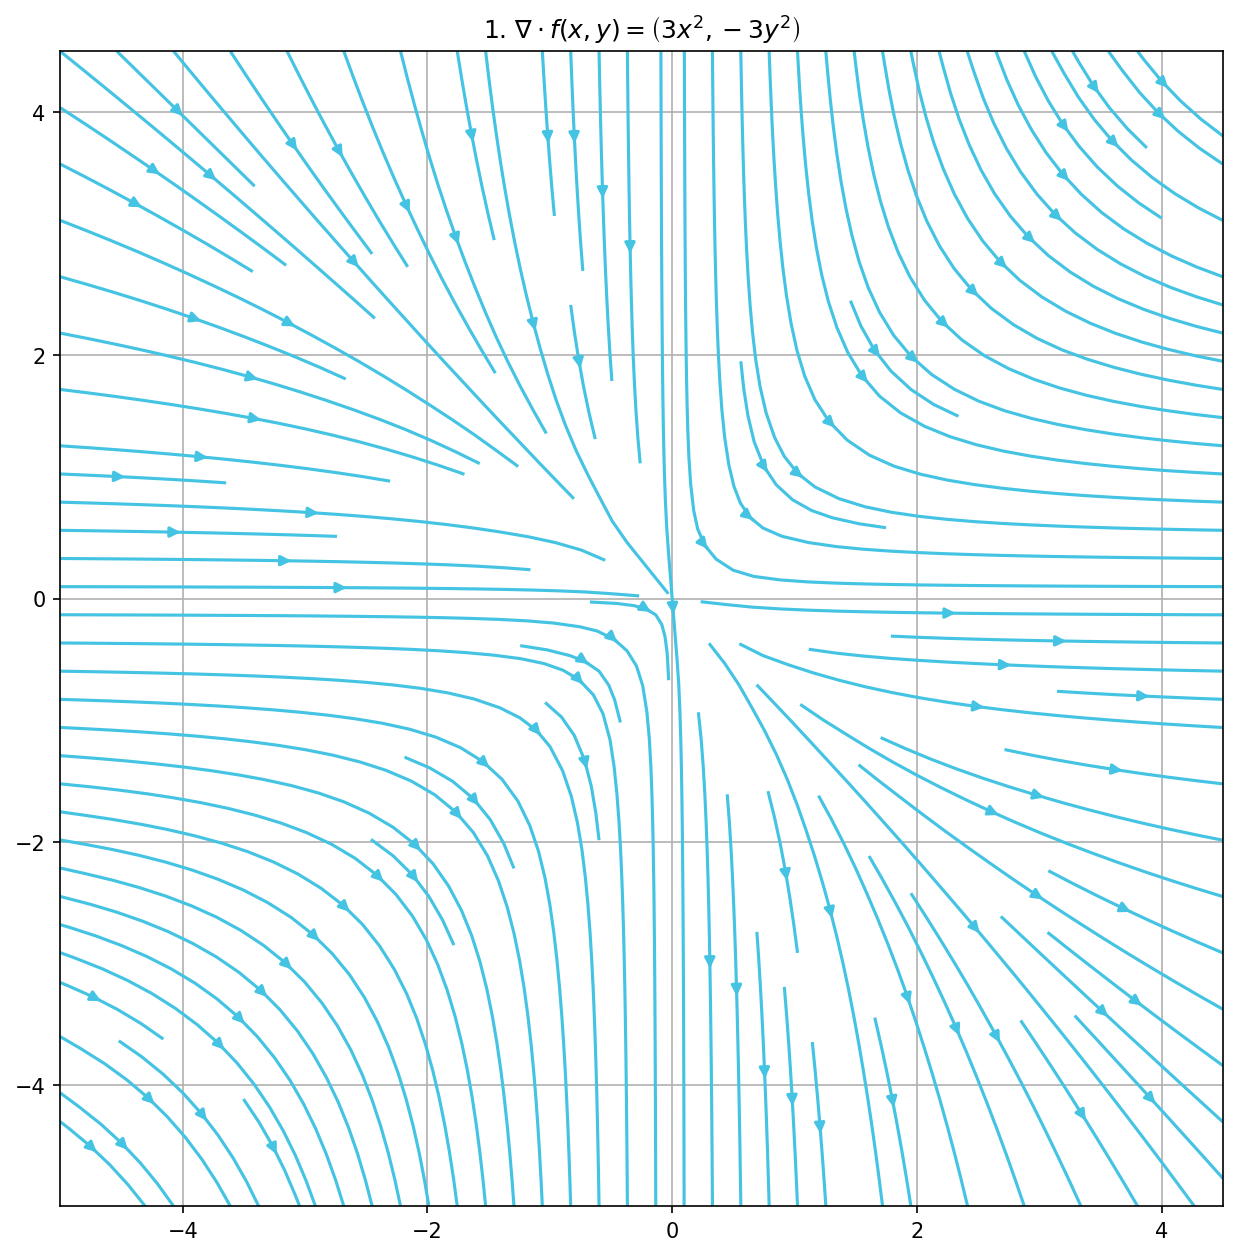
\includegraphics[width=0.65\linewidth]{Images/Ejercicio_1_Vectorial.png}
    \caption{Campo Vectorial 1.}
    \label{fig:vect1}
\end{figure}

\begin{lstlisting}[language=Python]
# 1. Definimos los ejes (vectores 1D)
range_val = np.linspace(-20, 20, 50)

# 2. CREAMOS LA MALLA
x = np.outer(np.linspace(-3, 3, 100), np.ones(100))
#Vector Transpuesta
y = x.copy().T
# 3. Calculamos Z usando las matrices
z = -x**3 + y**3

# 4. Graficamos (usando una proyeccion 3D)
fig = plt.figure(figsize=(10, 8))
ax = plt.axes(projection='3d') # Importante definir que es 3D

ax.plot_surface(x, y, z, cmap='inferno')
ax.set_title(r"2. $f(x,y) = -x^3+y^3$", fontsize=16, color='navy', pad=20)

fig.savefig('Ejercicio_2_Escalar.png', dpi=150, bbox_inches='tight')

plt.show()
\end{lstlisting}
\begin{figure}[H]
    \centering
    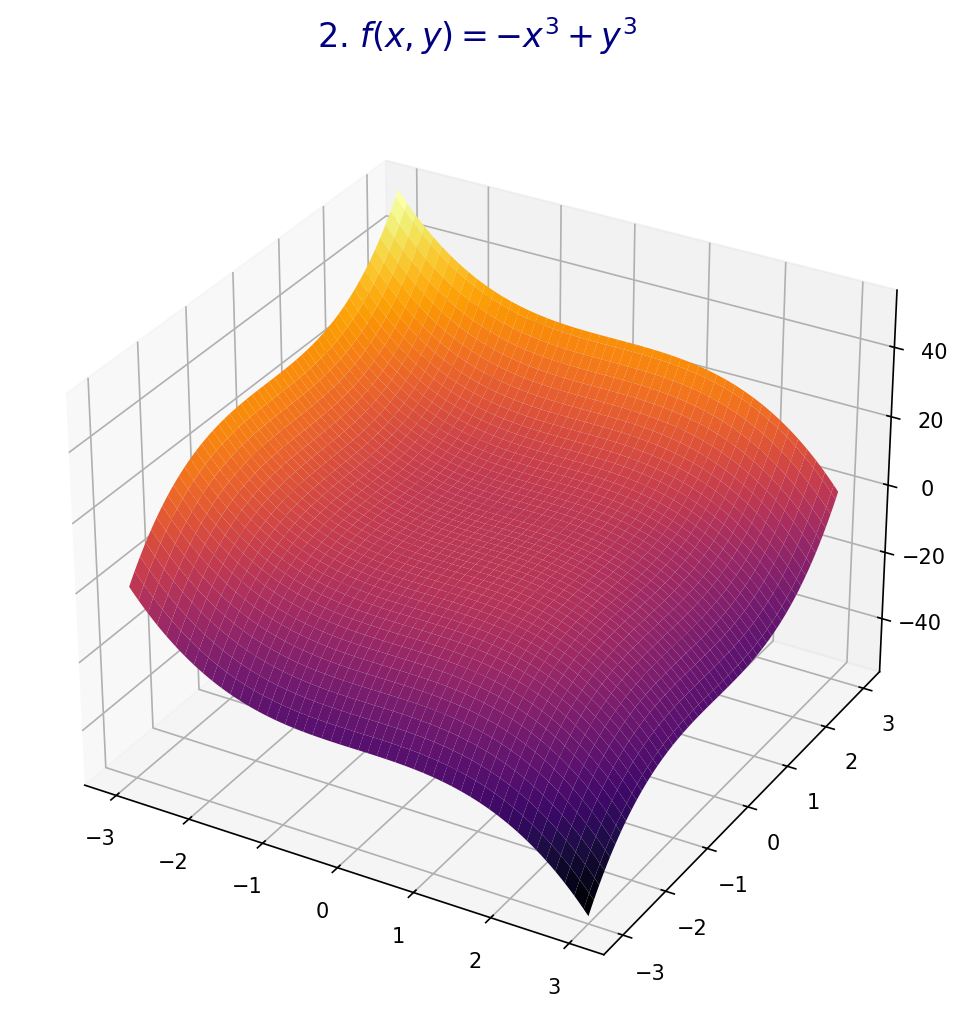
\includegraphics[width=0.65\linewidth]{Images/Ejercicio_2_Escalar.png}
    \caption{Función Escalar 2.}
    \label{fig:Esc2}
\end{figure}
\begin{lstlisting}[language=Python]
# 1D arrays
x = np.arange(-5,5,0.5)
y = np.arange(-5,5,0.5)

# Meshgrid
X,Y = np.meshgrid(x,y)

# Assign vector directions
fx = -3 * X**2
fy = 3 * Y**2

# Depict illustration
fig = plt.figure(figsize=(10, 10))
plt.streamplot(X,Y,fx,fy, density=1.4, linewidth=None, color='#C7C481')
plt.title(r'2. $ \nabla f(x,y) = \left(-3x^2 , 3y^2 \right) $')

# Show plot with grid
plt.grid()
fig.savefig('Ejercicio_2_Vectorial.png', dpi=150, bbox_inches='tight')
plt.show()
\end{lstlisting}
\begin{figure}[H]
    \centering
    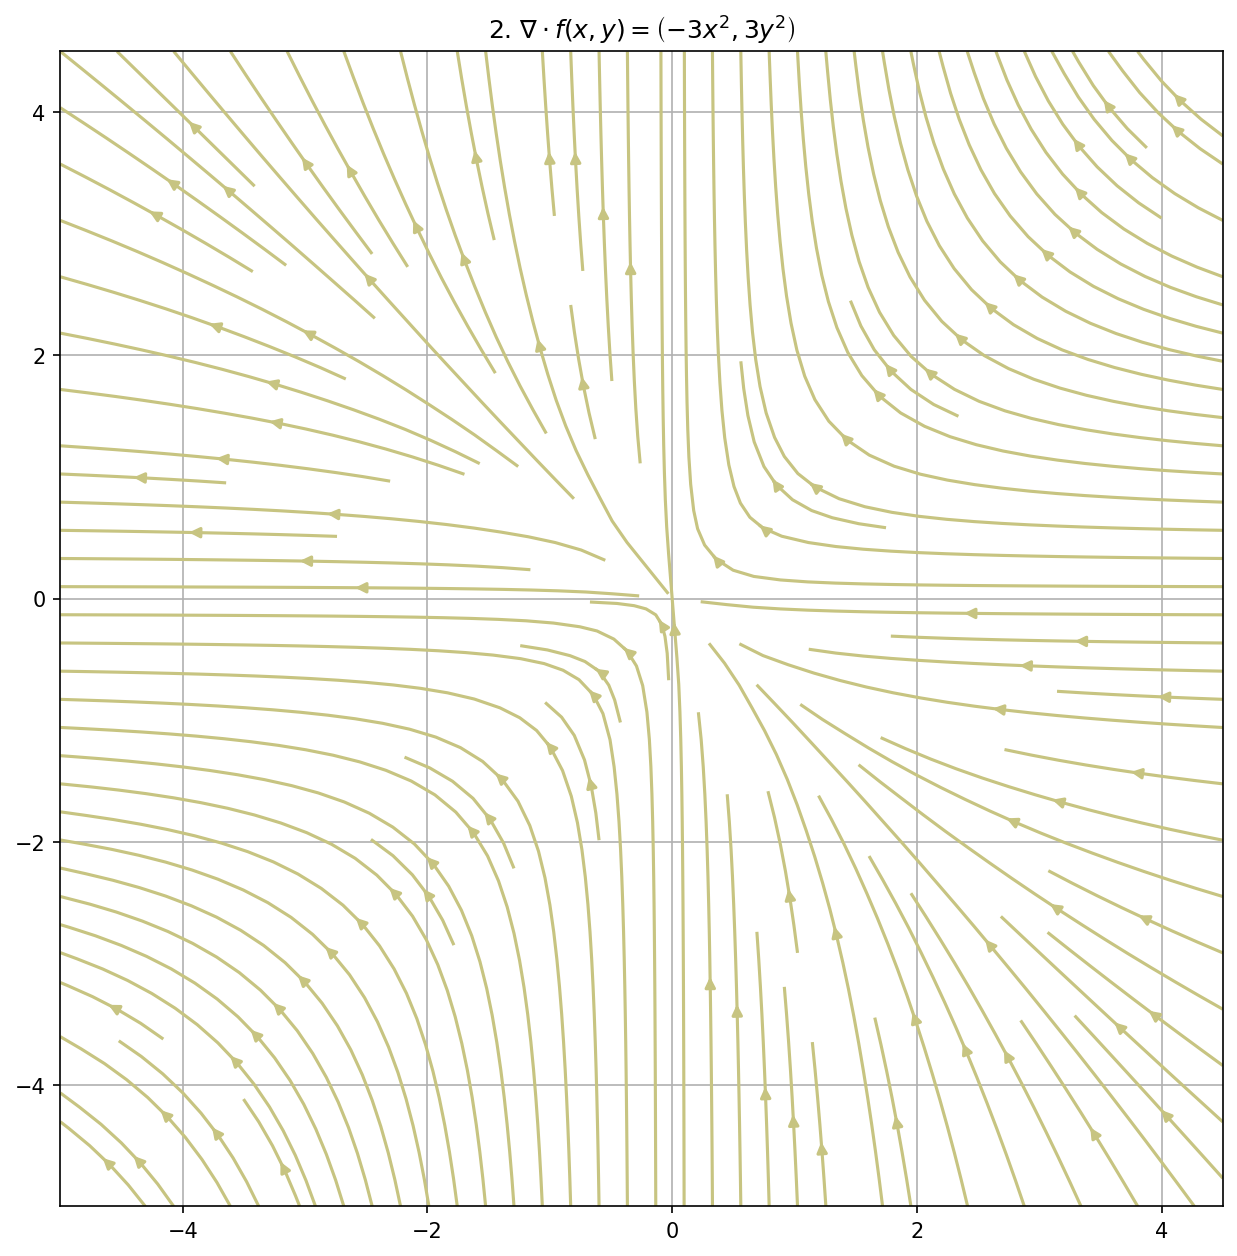
\includegraphics[width=0.65\linewidth]{Images/Ejercicio_2_Vectorial.png}
    \caption{Campo Vectorial 2.}
    \label{fig:vect2}
\end{figure}



\begin{lstlisting}[language=Python]
# 1. Definimos los ejes (vectores 1D)
range_val = np.linspace(-20, 20, 50)

# 2. CREAMOS LA MALLA

x = np.outer(np.linspace(-3, 3, 50), np.ones(50))
#Vector Transpuesta
y = x.copy().T

# 3. Calculamos Z usando las matrices
Z = x**2 * y**2 - np.sin(x * y)

# 4. Graficamos (usando una proyeccion 3D)
fig = plt.figure(figsize=(10, 8))
ax = plt.axes(projection='3d') # Importante definir que es 3D

ax.plot_surface(x, y, Z, cmap='inferno')
ax.view_init(elev=70)
ax.set_title(r"3. $f(x,y) = x^2 y^2 -\sin{(xy)}$", fontsize=16, color='navy', pad=20)

fig.savefig('Ejercicio_3_Escalar.png', dpi=150, bbox_inches='tight')

plt.show()
\end{lstlisting}
\begin{figure}[H]
    \centering
    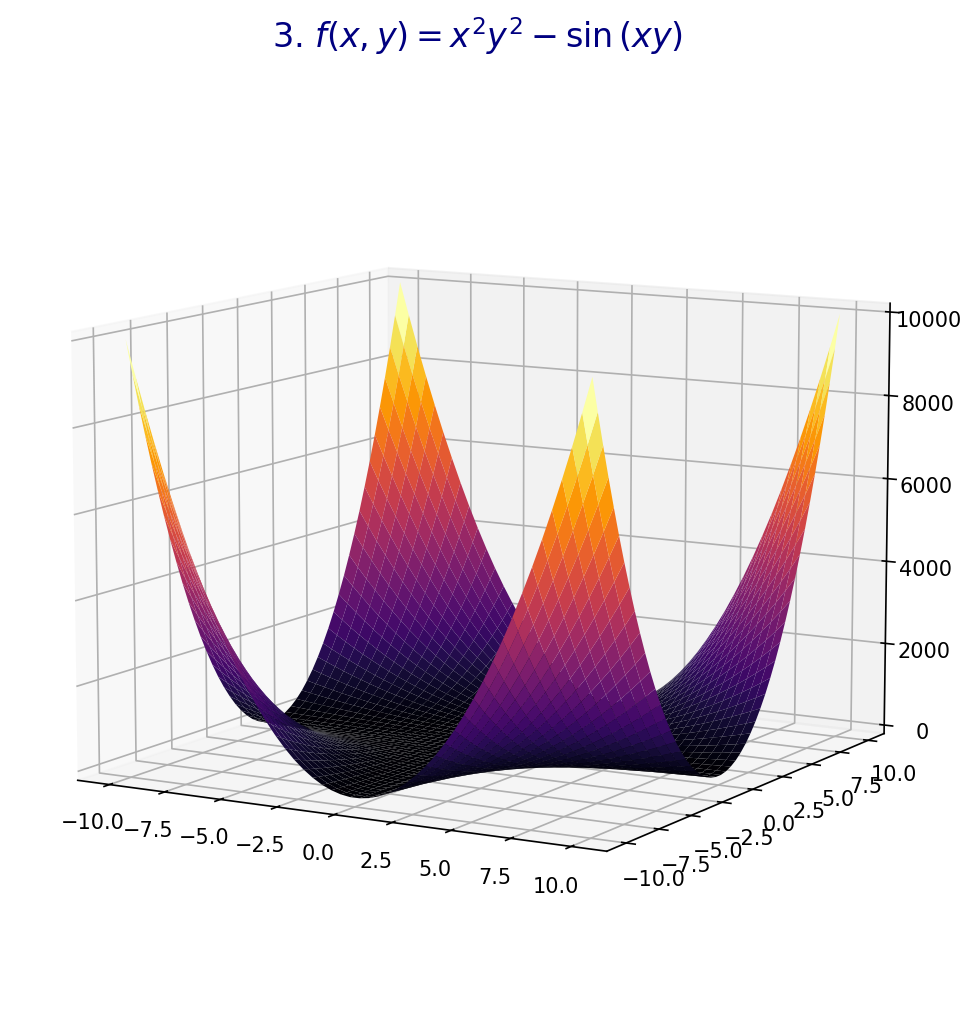
\includegraphics[width=0.65\linewidth]{Images/Ejercicio_3_Escalar.png}
    \caption{Función Escalar 3.}
    \label{fig:Esc3}
\end{figure}
\begin{lstlisting}[language=Python]
# 1D arrays
x = np.arange(-5,5,0.5)
y = np.arange(-5,5,0.5)

# Meshgrid
X,Y = np.meshgrid(x,y)

# Assign vector directions
fx = 2 * X * Y**2 - Y * np.cos(X * Y)
fy = 2 * X**2 * Y - X * np.cos(X * Y)

# Depict illustration
fig = plt.figure(figsize=(10, 10))
plt.streamplot(X,Y,fx,fy, density=1.4, linewidth=None, color='#C45CC4')
plt.title(r'3. $ \nabla f(x,y) = \left(2xy^2-y\cos(xy) , 2x^2y-x\cos(xy) \right) $')

# Show plot with grid
plt.grid()
fig.savefig('Ejercicio_3_Vectorial.png', dpi=150, bbox_inches='tight')
plt.show()
\end{lstlisting}
\begin{figure}[H]
    \centering
    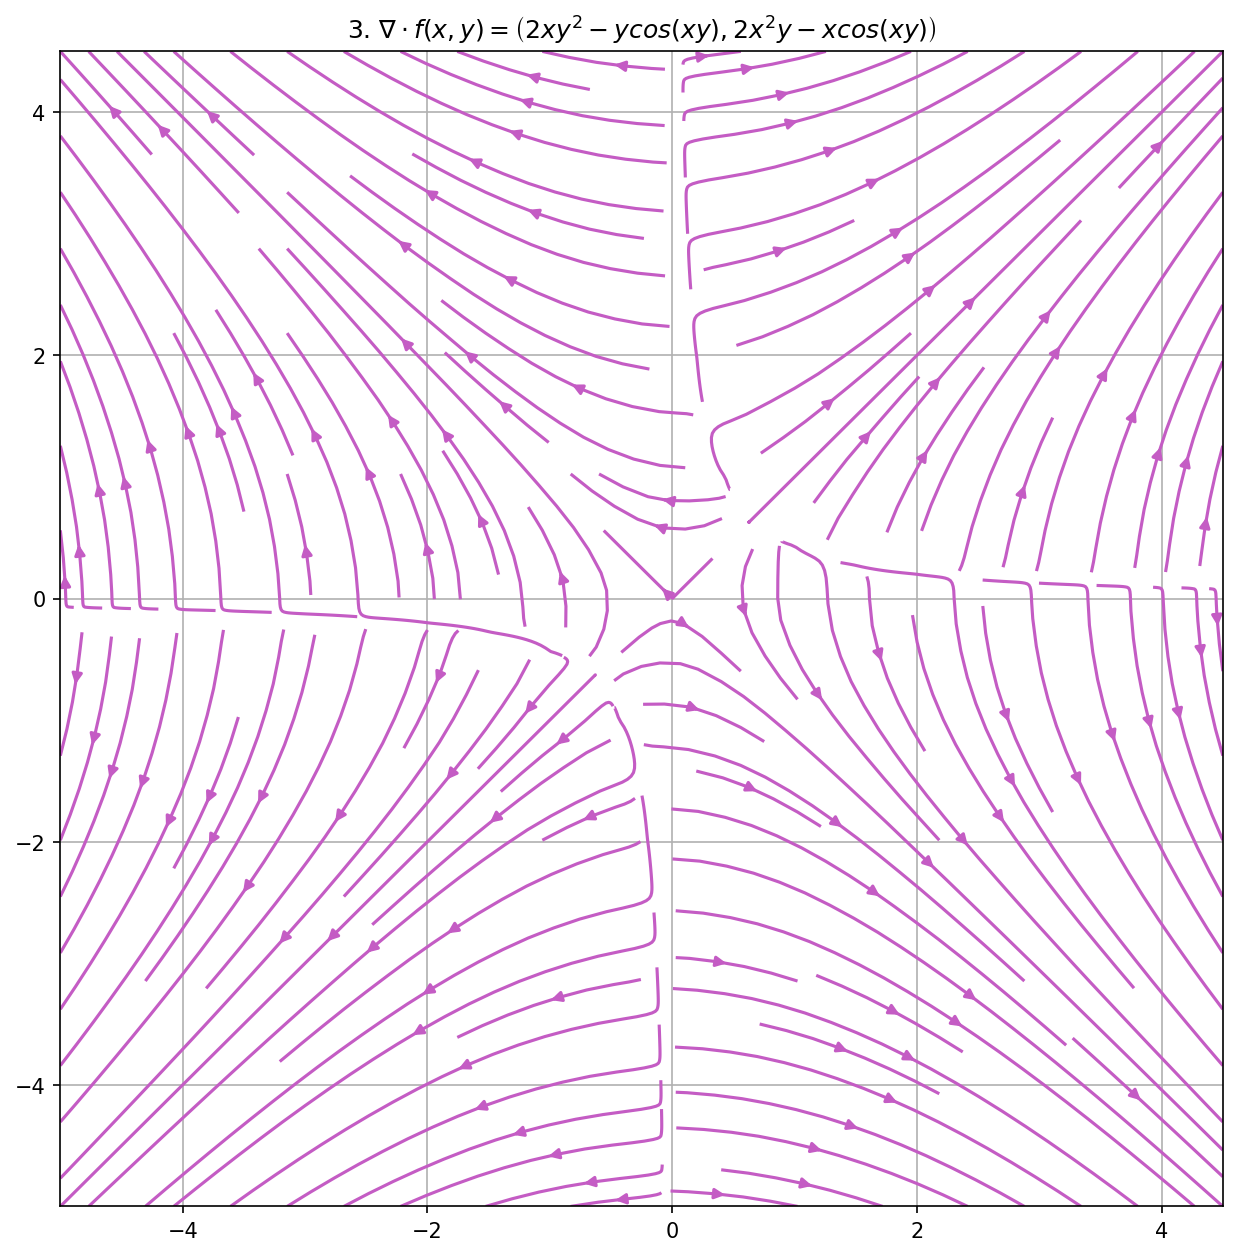
\includegraphics[width=0.65\linewidth]{Images/Ejercicio_3_Vectorial.png}
    \caption{Campo Vectorial 3.}
    \label{fig:vect3}
\end{figure}

\begin{lstlisting}[language=Python]
# 1. Definimos los ejes (vectores 1D)
range_val = np.linspace(-20, 20, 50)

# 2. CREAMOS LA MALLA
x = np.outer(np.linspace(-10, 10, 500), np.ones(500))
y = x.copy().T

# 3. Calculamos Z usando las matrices
z = np.\sin(x) * np.\cos(y) - np.cos(y**2)

# 4. Graficamos (usando una proyeccion 3D)
fig = plt.figure(figsize=(10, 8))
ax = plt.axes(projection='3d') # Importante definir que es 3D

ax.plot_surface(x, y, z, cmap='inferno')
ax.view_init(elev=60)
 
ax.set_title(r"4. $f(x,y) = \sin{(x)}\cos{(y)} -\cos{(y^2)}$", fontsize=16, color='navy', pad=20)

fig.savefig('Ejercicio_4_Escalar.png', dpi=150, bbox_inches='tight')

plt.show()
\end{lstlisting}
\begin{figure}[H]
    \centering
    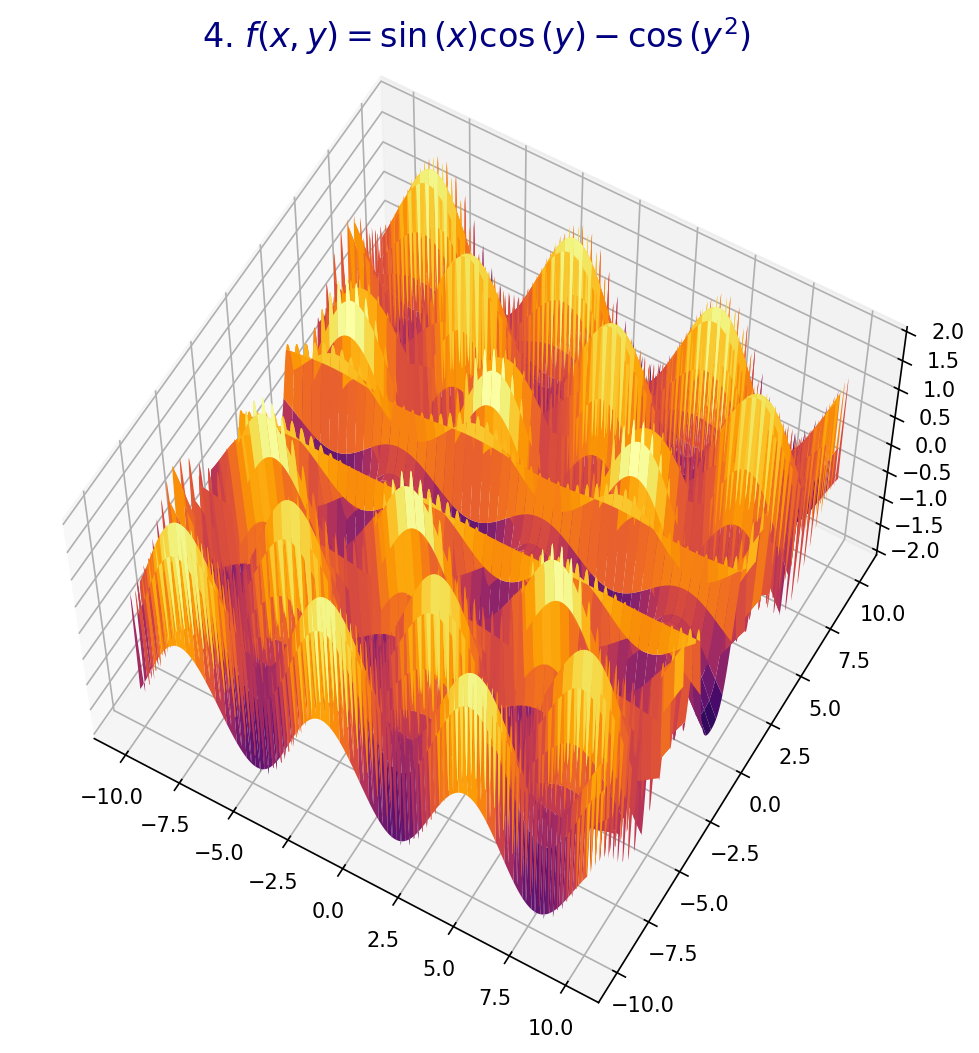
\includegraphics[width=0.65\linewidth]{Images/Ejercicio_4_Escalar.png}
    \caption{Función Escalar 4.}
    \label{fig:Esc4}
\end{figure}
\begin{lstlisting}[language=Python]
# 1D arrays
x = np.arange(-5,5,0.5)
y = np.arange(-5,5,0.5)

# Meshgrid
X,Y = np.meshgrid(x,y)

# Assign vector directions
fx = np.\cos(x) * np.\cos(y)
fy = 2 * Y * np.sin(Y**2) - np.\sin(x) * np.\sin(y)

# Depict illustration
fig = plt.figure(figsize=(10, 10))
plt.streamplot(X,Y,fx,fy, density=1.4, linewidth=None, color='#C45C5C')
plt.title(r'4. $ \nabla f(x,y) = \left(\cos(x)\cos(y), 2ysin(y^2)-\sin(x)\sin(y)) \right)$')

# Show plot with grid
plt.grid()
fig.savefig('Ejercicio_4_Vectorial.png', dpi=150, bbox_inches='tight')
plt.show()
\end{lstlisting}
\begin{figure}[H]
    \centering
    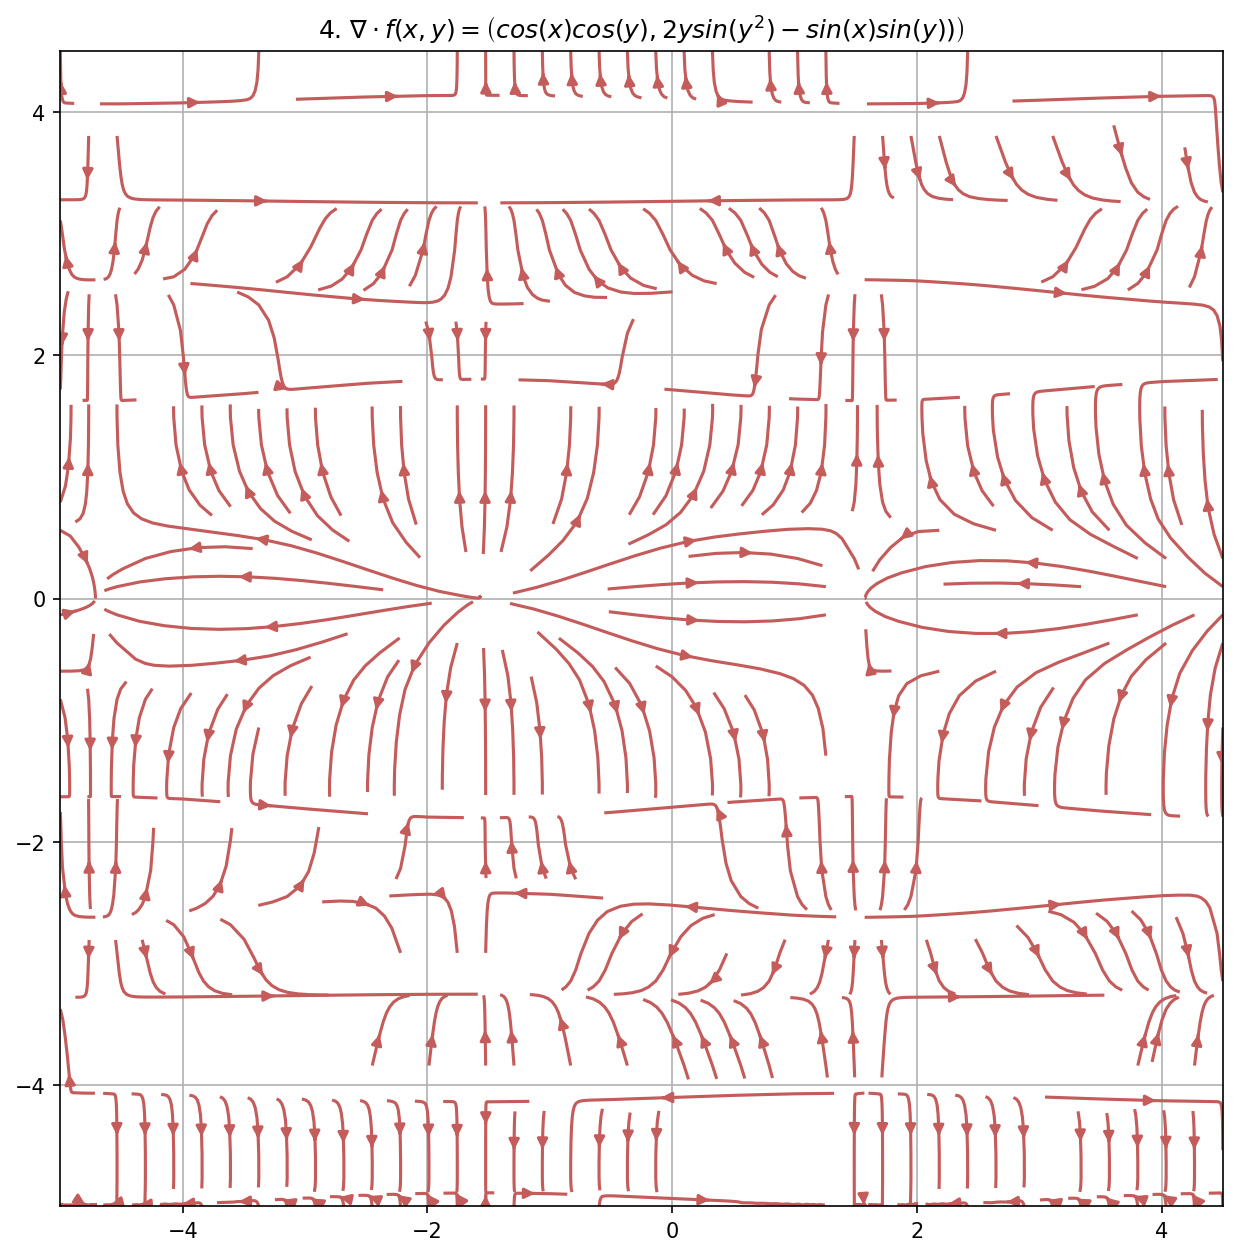
\includegraphics[width=0.65\linewidth]{Images/Ejercicio_4_Vectorial.png}
    \caption{Campo Vectorial 4.}
    \label{fig:vect4}
\end{figure}
\begin{lstlisting}[language=Python]
# 1. Definimos los ejes (vectores 1D)
range_val = np.linspace(-20, 20, 50)

# 2. CREAMOS LA MALLA
x = np.outer(np.linspace(-5, 5, 50), np.ones(50))
y = x.copy().T

# 3. Calculamos Z usando las matrices
z = x**3 +4* x**2 * y -5 * x * y**2 - y**3

# 4. Graficamos (usando una proyeccion 3D)
fig = plt.figure(figsize=(10, 8))
ax = plt.axes(projection='3d') # Importante definir que es 3D
ax.plot_surface(x, y, z, cmap='inferno')
ax.set_title(r"5. $f(x,y) = x^3+4x^2y-5xy^2-y^3 $", fontsize=16, color='navy', pad=20)
fig.savefig('Ejercicio_5_Escalar.png', dpi=150, bbox_inches='tight')

plt.show()
\end{lstlisting}
\begin{figure}[H]
    \centering
    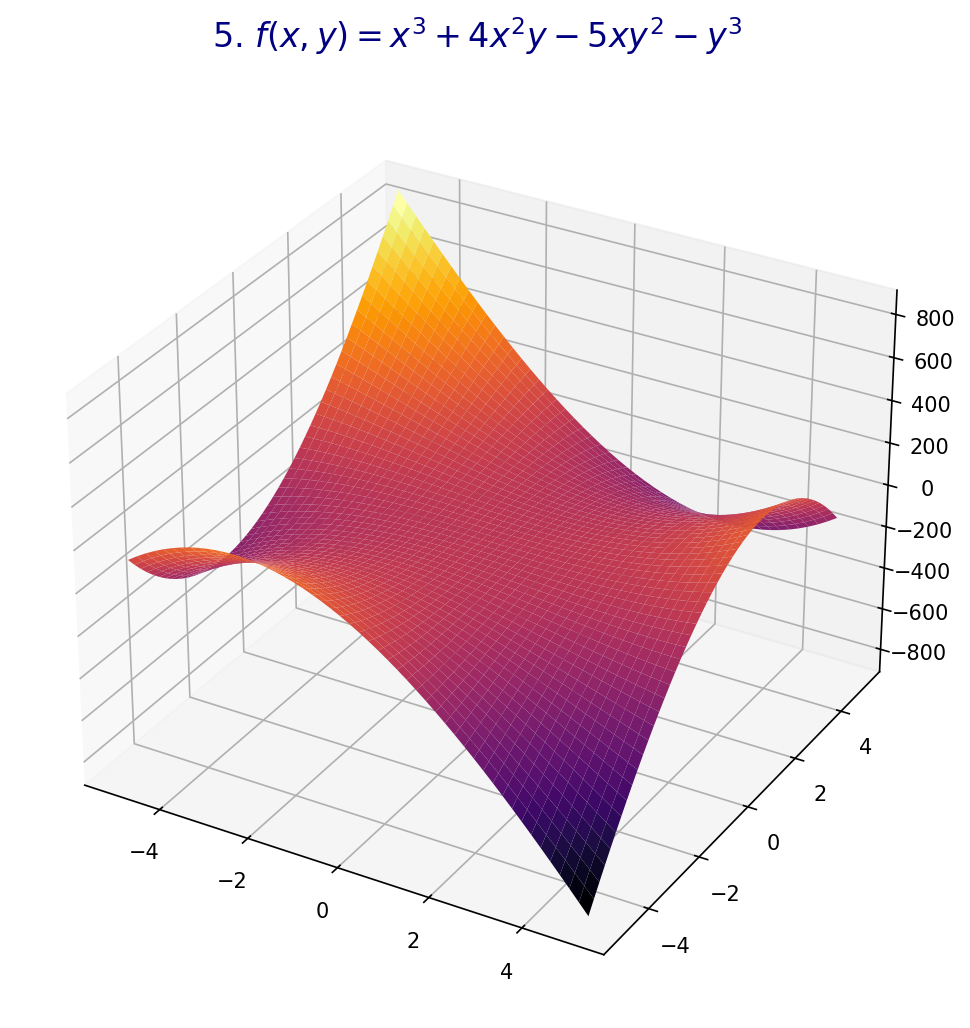
\includegraphics[width=0.65\linewidth]{Images/Ejercicio_5_Escalar.png}
    \caption{Función Escalar 5.}
    \label{fig:Esc5}
\end{figure}
\begin{lstlisting}[language=Python]
# 1D arrays
x = np.arange(-5,5,0.5)
y = np.arange(-5,5,0.5)

# Meshgrid
X,Y = np.meshgrid(x,y)

# Assign vector directions
fx = 3 * X**2 + 8 * X * Y - 5 * Y**2
fy = 4 * X**2 - 10 * X * Y - 3 * Y**2

# Depict illustration
fig = plt.figure(figsize=(10, 10))
plt.streamplot(X,Y,fx,fy, density=1.4, linewidth=None, color='#73C45C')
plt.title(r'5. $ \nabla f(x,y) = \left(3x^2+8xy-5y^2, 4x^2 -10xy - 3y^2\right)$')

# Show plot with grid
plt.grid()
fig.savefig('Ejercicio_5_Vectorial.png', dpi=150, bbox_inches='tight')
plt.show()
\end{lstlisting}
\begin{figure}[H]
    \centering
    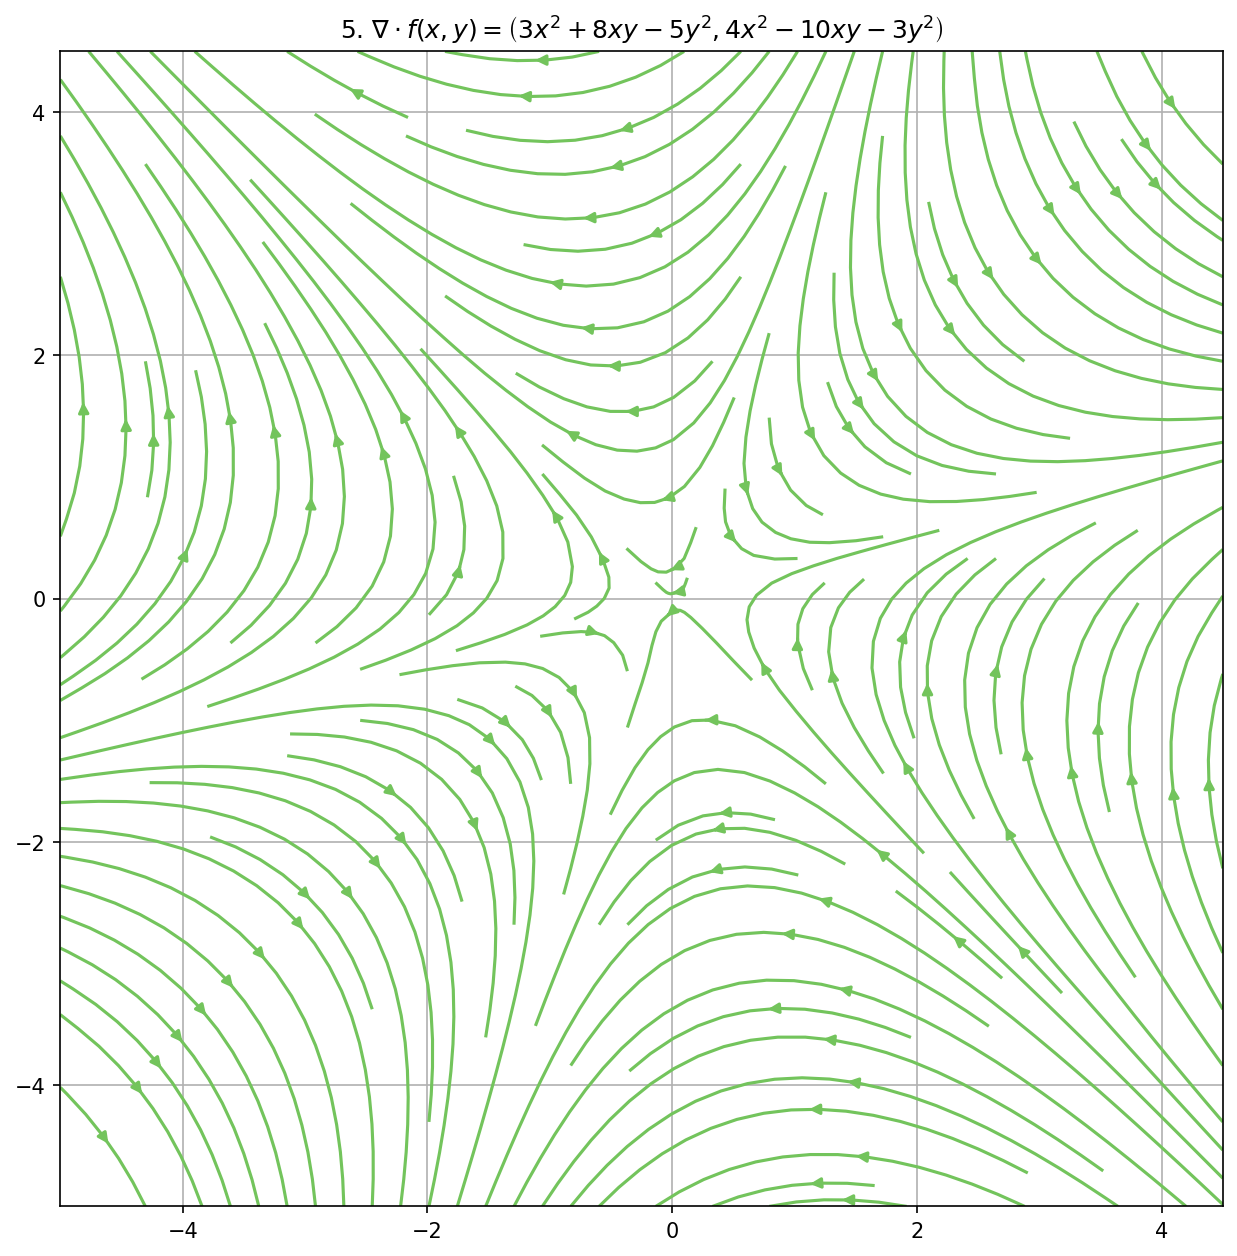
\includegraphics[width=0.65\linewidth]{Images/Ejercicio_5_Vectorial.png}
    \caption{Campo Vectorial 5.}
    \label{fig:vect5}
\end{figure}
\begin{lstlisting}[language=Python]
# 1. Definimos los ejes (vectores 1D)
range_val = np.linspace(-20, 20, 50)

# 2. CREAMOS LA MALLA
# X e Y ahora son matrices de 50x50
x = np.outer(np.linspace(-1, 1, 1000), np.ones(1000))
# Vector Transpuestas
y = x.copy().T

# 3. Calculamos Z usando las matrices
z = np.cos(x**3) + 4 * np.sin(x**2) * np.\cos(y) - 5 * x * y**2 + y**3

# 4. Graficamos (usando una proyeccion 3D)
fig, ax = plt.figure(figsize=(10, 8)), plt.axes(projection='3d') # Importante definir que es 3D


ax.plot_surface(x, y, z, cmap='inferno')
ax.view_init(elev=30, azim=45)

ax.set_title(r"6. $f(x,y) = \cos{(x^3)} -4\sin{(x^2)}\cos{(y)}-5xy^2+y^3$", fontsize=16, color='navy', pad=20)

fig.savefig('Ejercicio_6_Escalar.png', dpi=150, bbox_inches='tight')

plt.show()
\end{lstlisting}
\begin{figure}[H]
    \centering
    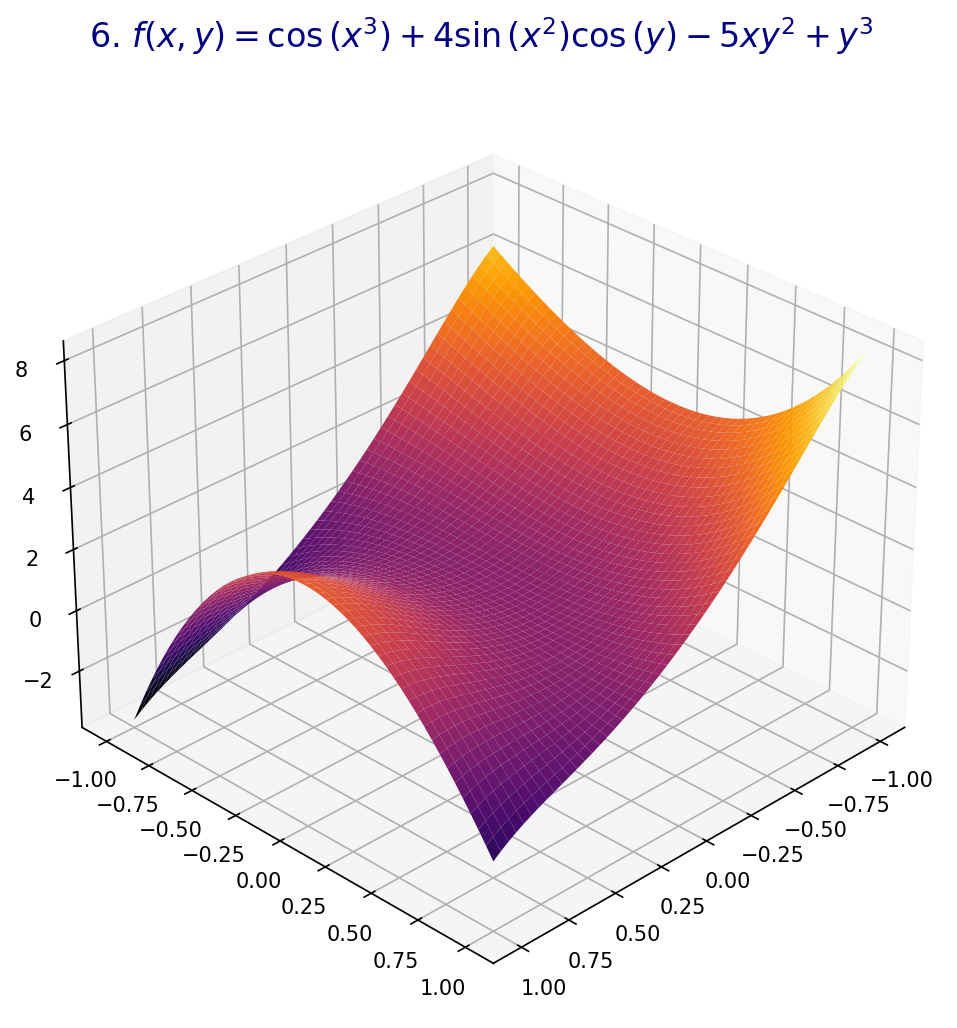
\includegraphics[width=0.65\linewidth]{Images/Ejercicio_6_Escalar.png}
    \caption{Función Escalar 6.}
    \label{fig:Esc6}
\end{figure}
\begin{lstlisting}[language=Python]
# 1D arrays
x = np.arange(-5,5,0.5)
y = np.arange(-5,5,0.5)

# Meshgrid
X,Y = np.meshgrid(x,y)

# Assign vector directions
fx = -3 * X**2 * np.sin(X**3) + 8 * X * np.cos(X**2) * np.\cos(y) -5 * Y**2
fy = -4 * np.sin(X**2) * np.\sin(y) - 10 * X * Y + 3 * Y**2

# Depict illustration
fig = plt.figure(figsize=(10, 10))
plt.streamplot(X,Y,fx,fy, density=1.4, linewidth=None, color='#722F37')
plt.title(r'6. $ \nabla f(x,y) = \left(-3x^2sin(x^3) + 8xcos(x^2)\cos(y) - 5y^2, -4sin(x^2)\sin(y)-10xy + 3y^2\right)$')

# Show plot with grid
plt.grid()
fig.savefig('Ejercicio_6_Vectorial.png', dpi=150, bbox_inches='tight')
plt.show()
\end{lstlisting}
\begin{figure}[H]
    \centering
    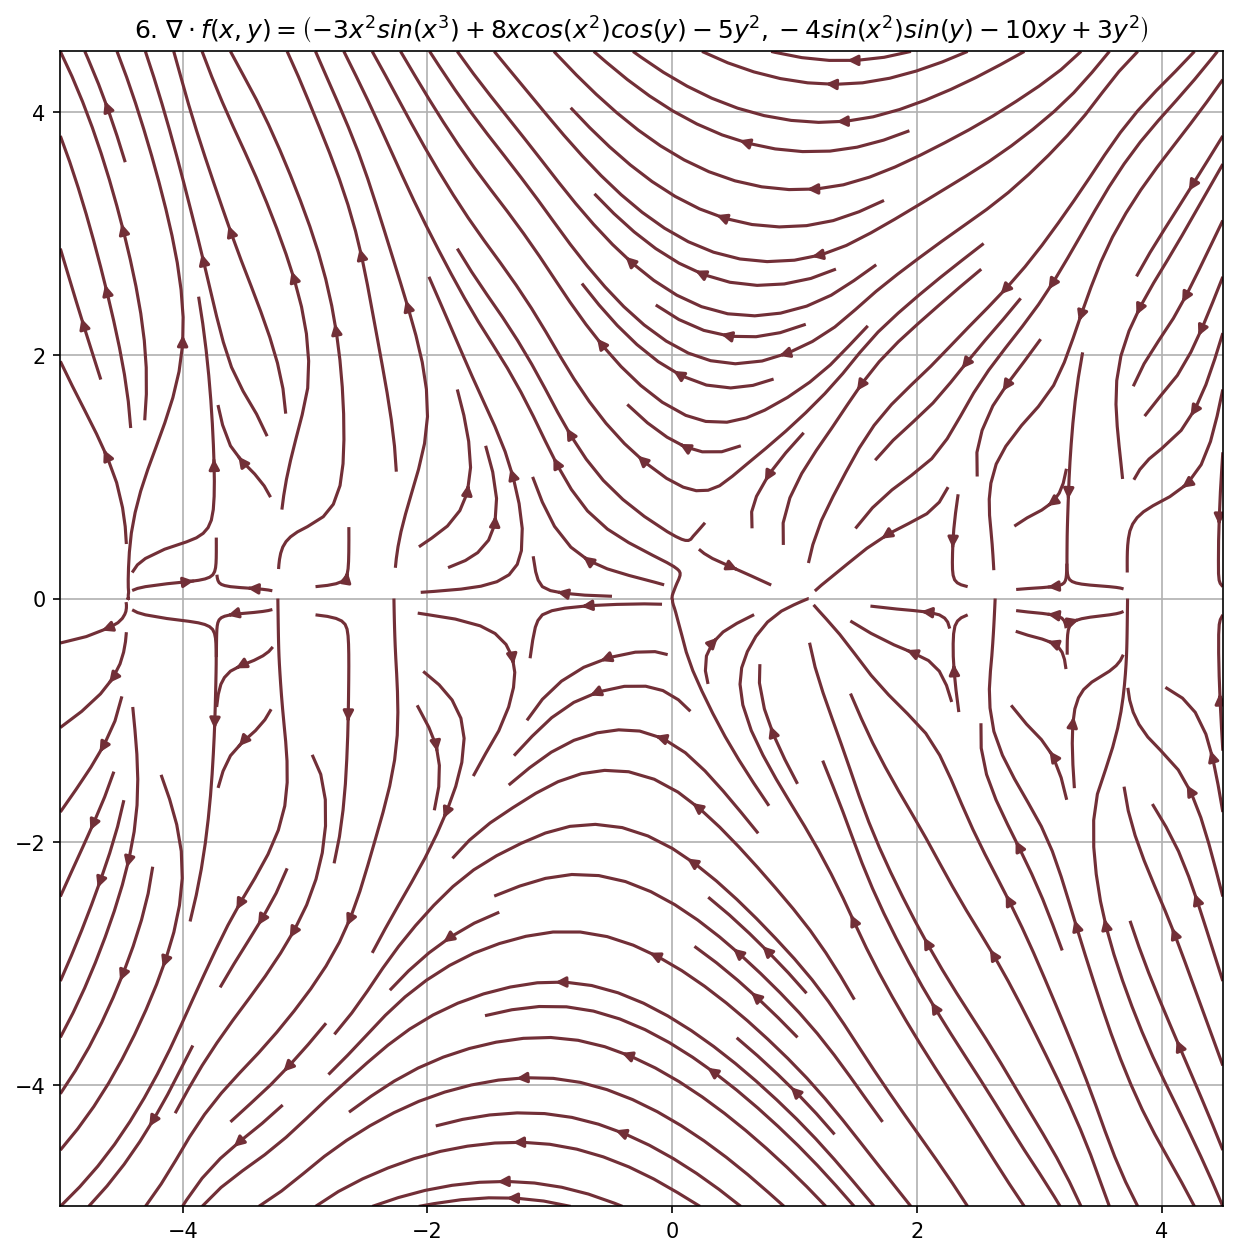
\includegraphics[width=0.65\linewidth]{Images/Ejercicio_6_Vectorial.png}
    \caption{Campo Vectorial 6.}
    \label{fig:vect6}
\end{figure}
\begin{thebibliography}{4}

\bibitem{marsden_tromba_calculo_vectorial}
Marsden, Jerrold E.; Tromba, Anthony J.
\textit{Cálculo vectorial}.
Traducción de Manuel López Mateos con la colaboración de Sergio Adarve D.
Addison-Wesley Iberoamericana, 1991.
\end{thebibliography}


\end{document}